\section{Resultados}

\subsection{Gap por modelo}
% Os 10 gaps são negativos, com IC abaixo de 0 (asserção em build_numbers), e o maior p de Holm; média dos modelos (pooled).
\todo{gaps por modelo, IC e maior p de Holm}
% Tabela 1 (gerada): por modelo e benchmark, taxa em texto, gap [IC], contraste logit [IC] e razão de tokens.
\todo{leitura da Tabela 1}
% Leitura ordinal por causa do piso, com o Qwen2.5-VL (floor_ceiling); leave-one-project-out no CoderUJB, numa frase (lopo).
\todo{piso e leave-one-project-out}

\begin{figure}[t]
  \centering
  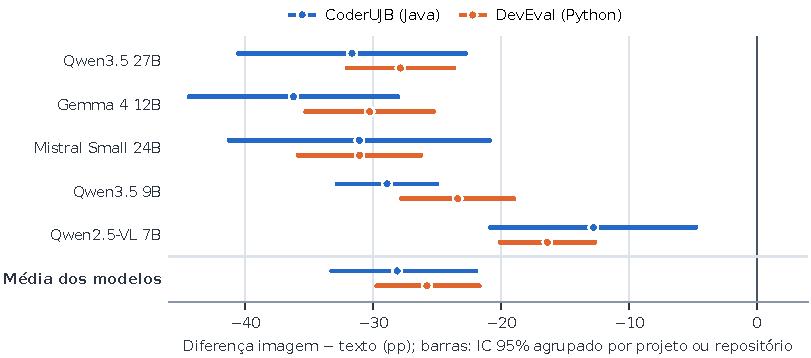
\includegraphics[width=\linewidth]{figures/fig_gap}
  \caption{\todo{legenda da Figura 1: gap imagem menos texto por modelo aberto e média dos modelos, IC 95\% agrupado por projeto}}
  \label{fig:gap}
\end{figure}

\begin{table}[t]
  \centering
  \caption{\todo{legenda da Tabela 1}}
  \label{tab:gaps}
  \resizebox{\linewidth}{!}{\begin{tabular}{lrrcrcr}
\toprule
Modelo & Texto (\%) & Gap (pp) & IC 95\% & Contraste (logit) & IC 95\% & Razão de tokens \\
\midrule
\multicolumn{7}{l}{\emph{CoderUJB, 136 itens}} \\
Qwen3.5 27B & 54,0 & \ensuremath{-}31,7 & [\ensuremath{-}40,5; \ensuremath{-}22,8] & \ensuremath{-}4,05 & [\ensuremath{-}4,81; \ensuremath{-}3,29] & 0,47 \\
Gemma 4 12B & 44,5 & \ensuremath{-}36,2 & [\ensuremath{-}44,4; \ensuremath{-}28,1] & \ensuremath{-}5,71 & [\ensuremath{-}6,63; \ensuremath{-}4,80] & 0,18 \\
Mistral Small 3.2 24B & 43,4 & \ensuremath{-}31,1 & [\ensuremath{-}41,3; \ensuremath{-}20,9] & \ensuremath{-}4,51 & [\ensuremath{-}5,31; \ensuremath{-}3,72] & 0,70 \\
Qwen3.5 9B & 41,4 & \ensuremath{-}28,9 & [\ensuremath{-}32,8; \ensuremath{-}25,0] & \ensuremath{-}4,27 & [\ensuremath{-}5,06; \ensuremath{-}3,48] & 0,47 \\
Qwen2.5-VL 7B & 22,2 & \ensuremath{-}12,8 & [\ensuremath{-}20,8; \ensuremath{-}4,8] & \ensuremath{-}2,37 & [\ensuremath{-}3,14; \ensuremath{-}1,61] & 0,66 \\
\emph{Média dos modelos} &  & \ensuremath{-}28,1 & [\ensuremath{-}33,2; \ensuremath{-}22,0] &  &  &  \\
\midrule
\multicolumn{7}{l}{\emph{DevEval, 859 itens}} \\
Qwen3.5 27B & 53,5 & \ensuremath{-}27,9 & [\ensuremath{-}32,0; \ensuremath{-}23,7] & \ensuremath{-}4,34 & [\ensuremath{-}4,69; \ensuremath{-}3,99] & 0,47 \\
Gemma 4 12B & 46,1 & \ensuremath{-}30,3 & [\ensuremath{-}35,3; \ensuremath{-}25,3] & \ensuremath{-}5,19 & [\ensuremath{-}5,57; \ensuremath{-}4,81] & 0,21 \\
Mistral Small 3.2 24B & 48,3 & \ensuremath{-}31,1 & [\ensuremath{-}35,9; \ensuremath{-}26,3] & \ensuremath{-}4,95 & [\ensuremath{-}5,31; \ensuremath{-}4,59] & 0,69 \\
Qwen3.5 9B & 41,2 & \ensuremath{-}23,4 & [\ensuremath{-}27,8; \ensuremath{-}19,0] & \ensuremath{-}3,86 & [\ensuremath{-}4,20; \ensuremath{-}3,52] & 0,47 \\
Qwen2.5-VL 7B & 30,2 & \ensuremath{-}16,4 & [\ensuremath{-}20,1; \ensuremath{-}12,7] & \ensuremath{-}3,10 & [\ensuremath{-}3,44; \ensuremath{-}2,77] & 0,65 \\
\emph{Média dos modelos} &  & \ensuremath{-}25,8 & [\ensuremath{-}29,7; \ensuremath{-}21,7] &  &  &  \\
\bottomrule
\end{tabular}
}
\end{table}

\subsection{Fonte e tokens}
% 14 px supera 12 px por 4,1 a 8,8 pp, com IC acima de 0, para o Qwen3.5 27B nos dois benchmarks e para o Mistral e o Qwen3.5 9B no DevEval (size_diffs; asserção sobre o conjunto); o Gemma economiza mais tokens e perde o mesmo em todo tamanho.
\todo{efeito do tamanho da fonte e economia de tokens}

\begin{figure}[t]
  \centering
  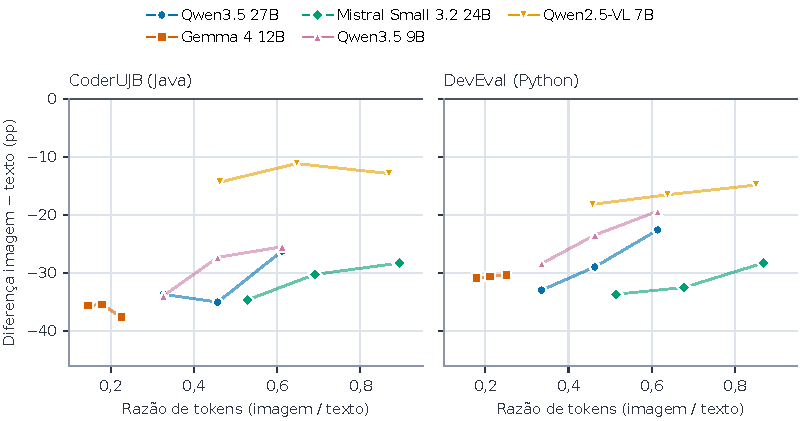
\includegraphics[width=\linewidth]{figures/fig_size_tokens}
  \caption{\todo{legenda da Figura 2: gap por tamanho contra a razão de tokens por tamanho, uma linha por modelo}}
  \label{fig:size-tokens}
\end{figure}

\subsection{A penalidade é igual entre itens e modelos?}
% Wald com 4 gl; DP item:condição com IC de perfil e razão sobre o DP de item; LRT como linha secundária; log-verossimilhança fora da amostra, positiva nas 10 dobras no DevEval e indistinguível de 0 no CoderUJB (asserção).
\todo{Wald, DP item:condição, LRT e fora da amostra}
% Correlação texto x imagem abaixo da referência e C de Pearson nos percentis 0,997 e 1,000; inclinação comum dividida por r e probit; nenhum item sobrevive ao BH (asserção); com 5 modelos não se estabelece uma segunda habilidade.
\todo{correlações, inclinação comum, probit, BH e limite de 5 modelos}

\begin{figure}[t]
  \centering
  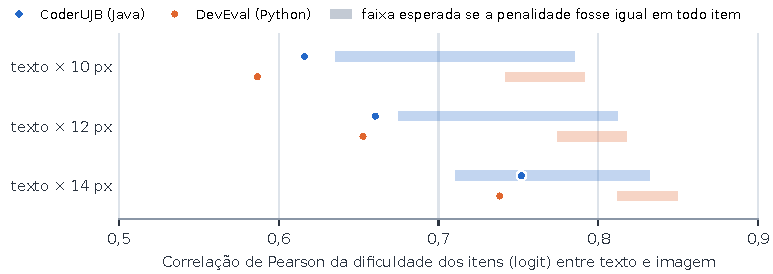
\includegraphics[width=\linewidth]{figures/fig_item_corr}
  \caption{\todo{legenda da Figura 3: correlação texto x imagem por tamanho contra a faixa de referência}}
  \label{fig:item-corr}
\end{figure}

\subsection{Confiabilidade e ordem}
% Confiabilidade de 1 e de 2 execuções e o G finito; CoderUJB a 12 px é instável; os três modelos do meio trocam de lugar (reliability.json; docs/paper/reliability.md como rascunho).
\todo{confiabilidade, G finito e troca de ordem}

\subsection{Contaminação}
% 25 e 149 itens com cópia (copied_items); 39 de 40 gaps encolhem e todos seguem negativos; controle acima do percentil 97,5 em 3 de 5 modelos por benchmark; os itens marcados perdem mais (associação e checagem fora do plano); concordância das duas flags (flag2).
\todo{contaminação: cópias, encolhimento, controle, itens marcados e flags}

\subsection{Exploratório}
% Claude perde de 1,7 a 6,2 pp; contraste c; teto no CoderUJB; itens marcados (claude main, glmm, contamination). Marcar como exploratório.
\todo{Claude, exploratório}
% Bloco 1: os erros a mais são de nome, com o exemplo _determine_alterations; o piloto não teve gap (block1/findings.md). Marcar como exploratório.
\todo{bloco 1, exploratório}
